%\section{Baseline Methods}
%\label{sec:method}
%In this section, we first formulate the tasks and propose two kinds of baseline methods in the two following sections, feature-based methods and LSTM-based methods.
%
\section{Linguistic Indicators of Relationships}
\label{sec:method}
 
Unlike other popular texts used in text classification datasets which 
have focused topics or similar styles (such as product comments), 
dialogues from movies are highly diverse with topics and linguistic
features: They can be casual, flexible, and about anything in the world.
Such diversity makes end-to-end learning 
infeasible on small-scale datasets, so we believe 
it is essential to guide the algorithm toward those ``critical'' 
aspects from human's perspective by manually defining and extracting 
indicative features from the dialogues.

To do this, we first make some observations on how humans make the inference. 
When measuring human performance (see \secref{subsec:human baseline}), 
we ask the volunteers to also highlight every part 
(e.g., words, punctuations, sentences) of the dialogues they found 
helpful in identifying relationships in the provided text. 
By analyzing those highlighted parts, 
we find that focused texts are similar across different volunteers. 
We summarize indicative features in conversation and show how to define and 
computationally extract them below.  
%Without those informative words, people observe tones, which can be reflected by punctuatiosn, modals, sentence types and so on. A higher level of comprehension is based on common sense. Take the sample in figure \ref{fig:instinct}: by asking "Will your father like me", we can infer that the speaker is about to meet his/her lover's family members and seems worried.

\subsection*{Address Terms} 
\label{sec:address terms}
Accounting for almost half of all the highlighted parts, address terms are
the most important indicators of relationship for humans. 
An informative address term such as ``dad'', ``darling'' will 
immediately make things clear, while a title before name like 
``Mr.'' at least tells us the relationship is formal. 
Previous study classifies address terms into 
3 categories~\cite{address-term}:
 names (e.g., Barack, Barack Hussein Obama), titles (e.g., Ms., Dr., Private) 
and placeholder names (e.g., dude, bro, asshole). It also provides 
lists of common title and placeholder lexicons, 
which are obtained by trained SVM classifier and filtered by humans. 
Based on their study, we design an address terms extractor which 
identifies words and syntactic patterns of interest through rule-matching. 
The confusion matrix on 1022 human-annotated test sentences are shown 
in figure \ref{fig:address}. 

\begin{figure}[t!]
	\centering
	\begin{subfigure}[t]{0.5\textwidth}
		\centering
		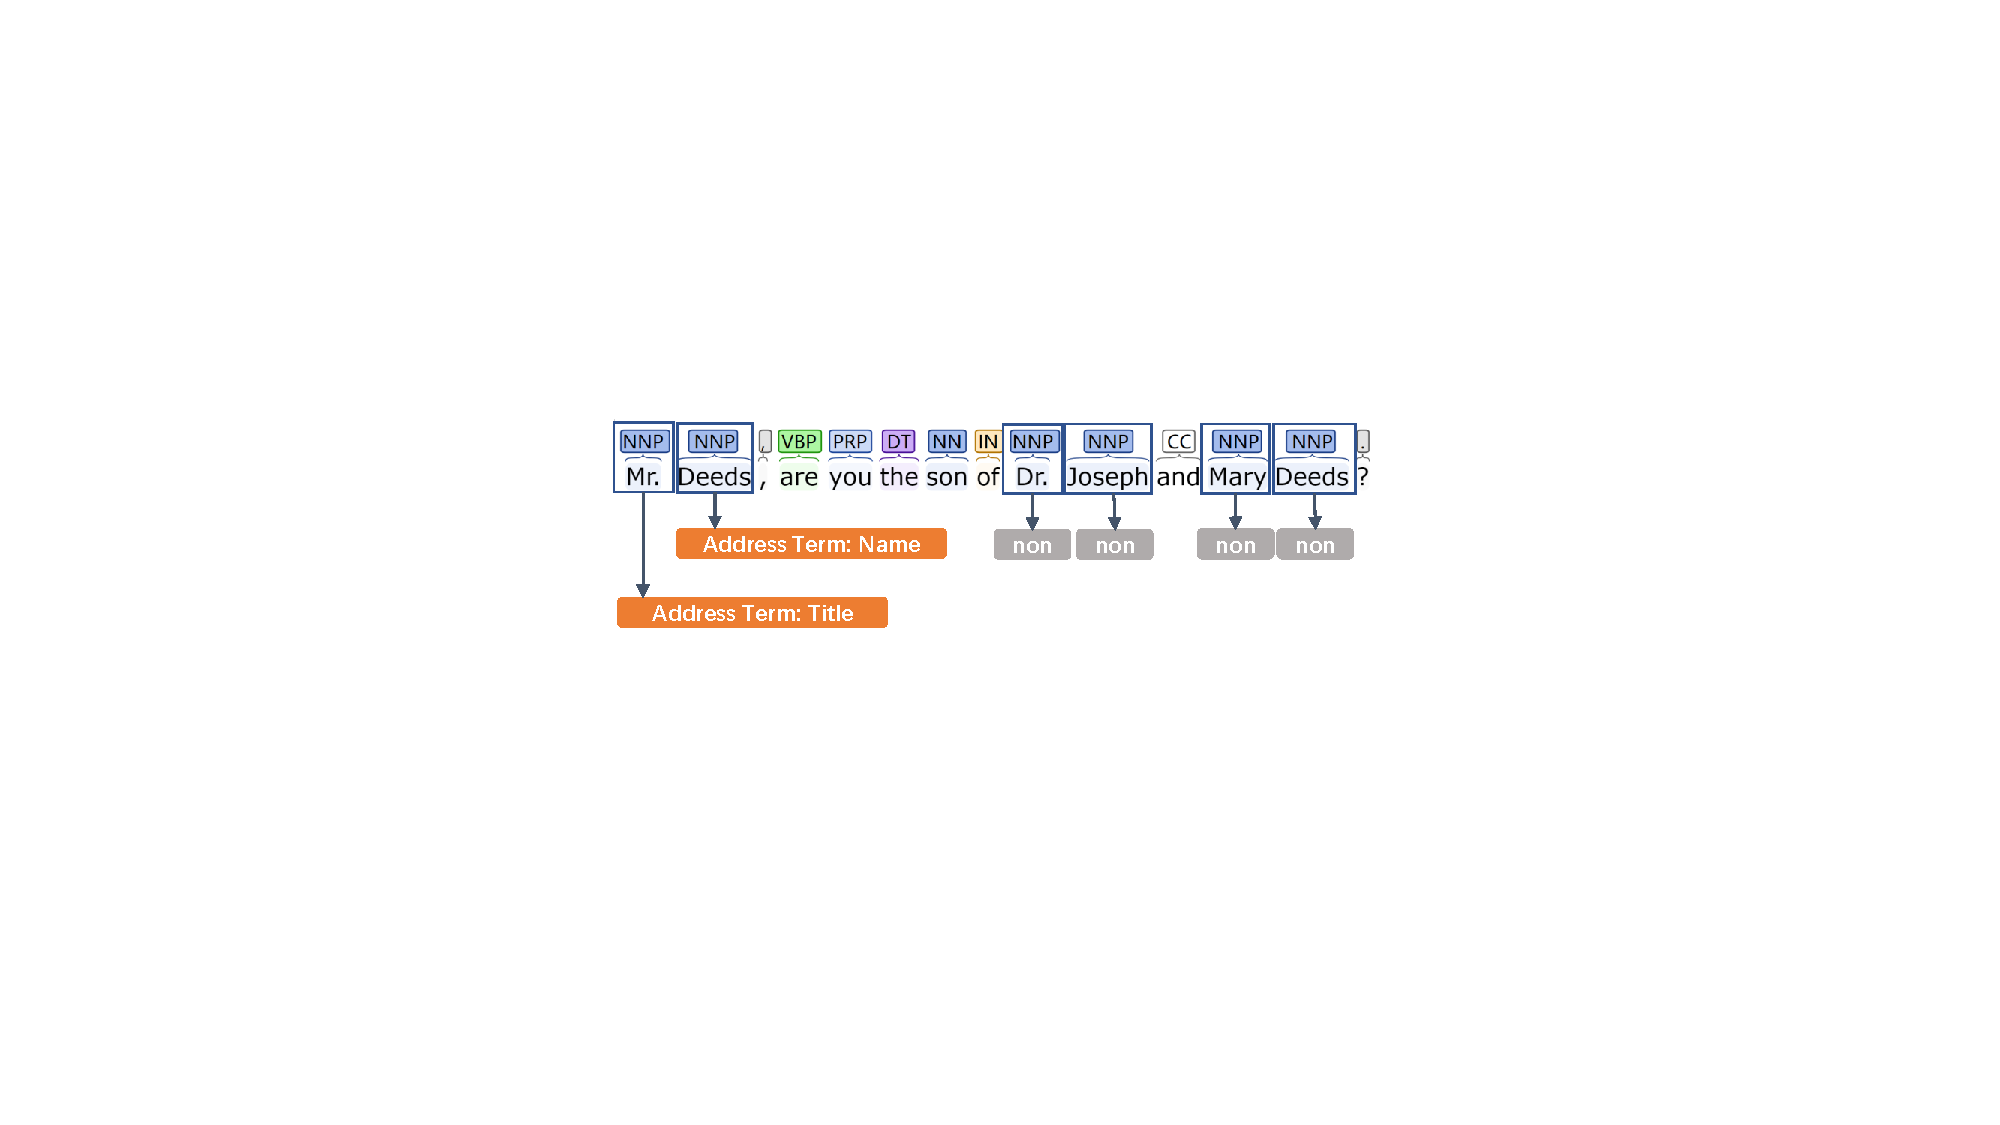
\includegraphics[height=1in]{add-sample.pdf}
		\caption{Example address-term annotation.}
	\end{subfigure}%
	\\
	\begin{subfigure}[t]{0.5\textwidth}
		\centering
		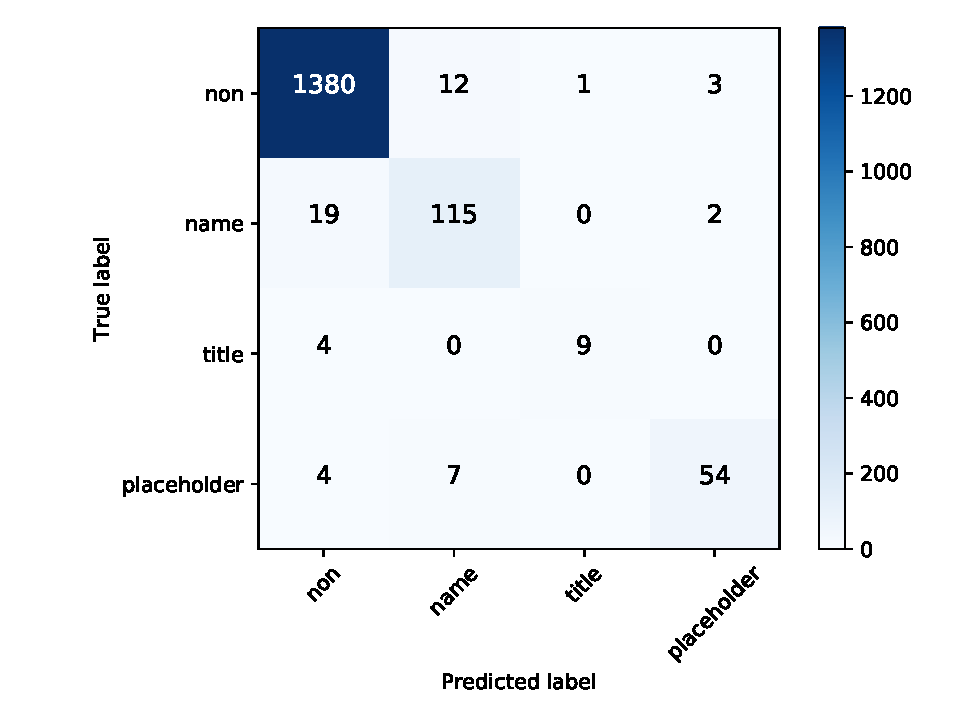
\includegraphics[height=2.3in]{confusion.pdf}
		\caption{The confusion matrix of our algorithm's predictions, compared with human annotations. Only nouns are considered.}
	\end{subfigure}
	\caption{Address-term extraction: rules and performance. Recall of our algorithm on all address terms(regardless of types) is 92.12\%.}\label{fig:address}
\end{figure}

We try two ways of vectorizing address terms: one-hot encoding and 
averaging word vectors (in which we used GloVe pretrained word 
vectors~\cite{glove}). To prevent the classifier from remembering specific person names, 
we vectorize only titles and placeholders, 
while for person names only the number of mentions are counted and
included as feature.

\subsection*{Key Words and Dependency Pairs} 
What the dialogue is about varies greatly across different 
relationships and thus can be a good indicator. For example, 
two people talking about kitchen utensils and dinner are likely 
family members. If words like ``authentication,'' ``report'' 
and ``office'' surface in a dialogue, 
a work place scene emerges in our mind. 
We first apply the topic modelling algorithm 
Latent Dirichlet Allocation(LDA)~\cite{LDA} with 
Term Frequency Inverse Document Frequency (TF-IDF) 
transfer on all of our processed dialogues ($36,728$ sessions, 
each session treated as a document), with Gensim~\cite{gensim}.
We adjust the number of topics ranging from $20$ to $500$, 
but the generated ``most related words'' in each topic don't
show obvious correlation, by human observation.
Another common approach is to generalize mentioned words into
their hypernyms in a taxonomy such as WordNet. 
%and use one at an appropriate level to represent the topic. 
We dismiss this approach because the hypernyms tend to be
too general to distinguish the words used by different relations.
%different relationships are not always in different subtrees 
%in the hierarchical structure of words. 
For example, the direct hypernyms of ``bedroom'' and ``boardroom'' 
are both ``room'', but the distinction is significant in our task.
\begin{table*}[th]
\small
\centering
	\begin{tabular}{|l|l|l|}
		\hline
		\multirow{2}{*}{Tokens}                                                      & family \textgreater workplace &  \begin{tabular}[c]{@{}l@{}}(punctuations removed or kept) she, dad, oh, honey, mother, \\house, love, okay, dear, sleep     \end{tabular}                                                                                                                                                                                                               \\ \cline{2-3} 
		& workplace \textgreater family & \begin{tabular}[c]{@{}l@{}}(punctuations removed) sir, got, (')ve, mr, man, yes, (')ll, right,\\  shit, little\\ (punctuations kept) . , ? 's n't ... 're -- sir got\end{tabular}                                                                                                  \\ \hline
		\multirow{2}{*}{Bi/Trigrams}                                                 & family \textgreater workplace & \begin{tabular}[c]{@{}l@{}}go to, all right, \textbf{you know}, \textbf{love you}, \textbf{what are you}, \textbf{with you}, \\ to bed, your mother, talk about, the phone\end{tabular}                                                                                                                                \\ \cline{2-3} 
		& workplace \textgreater family & \begin{tabular}[c]{@{}l@{}}you are, \textbf{in the}, \textbf{of the}, \textbf{on the}, \textbf{to the}, we re, yes sir, you think, \\ ve got, this is\end{tabular}                                                                                                                                                     \\ \hline
		\multirow{2}{*}{\begin{tabular}[c]{@{}l@{}}Dependency \\ Pairs\end{tabular}} & family \textgreater workplace & \begin{tabular}[c]{@{}l@{}}(case, `house', `in'), (nsubj, `want', `i'), (discourse, `god', `oh'), \\ (aux, `want', `do'), (nsubj, `okay', 'it')\end{tabular} \\ \cline{2-3} 
		& workplace \textgreater family & \begin{tabular}[c]{@{}l@{}}(discourse, `sir', `yes'), (nsubj, `got', `i'), (nsubj, `do', `i'), \\ (aux, `say', `did'), (nsubj, `have', `i')\end{tabular}      \\ \hline
	\end{tabular}
	\caption{Tokens, n-grams and dependency pairs that occurs 
significantly more frequently in one category than the other. 
The original texts are tokenized and lemmatized. 
%Stopwords and terms with document frequency 
%lower than 0.002 are ignored when extracting tokens features, 
%but are kept when extracting ngrams and dependency pair features. 
Punctuations are removed during tokenization unless otherwise stated. 
Items are separated by commas, but we use blanks instead in the second line where punctuations are kept, for clarity.}\label{table:dbow}
\end{table*}
%It's hard to figure out what the speakers are talking about, but both baseline volunteers worked on this sample got the right answer(workplace) with highest confidence, and highlighted the word 'order'. 

%After failure in topic modeling, we look into the dialogues and think twice about the role of ``topics'' in our inference. 
%As in the example of \figref{fig:instinct}, we don't really know 
%what they are talking about, 
%but on seeing the word ``order'' we know it's likely a workplace dialogue. 
To this end, we directly focus on indicative words. 
We define ``indicative'' by ``significantly more likely to occur in 
one relationship than the other''. 
First, we transfer all the dialogues into Bag-of-Words (BOW) vectors. 
Then we rank all the words by the difference in their 
relative frequencies in family dialogues and workplace dialogues. 
Formally, this is calculated by
\[
\frac{f_{family}(w)}{\sum_i f_{family}(w_i)} -
\frac{f_{work}(w)}{\sum_i f_{work}(w_i)},
\]
where $f_{family}(w)$ is the frequency of word $w$ in all family dialogues,
and  $f_{work}(w)$ is the frequency of $w$ in all workplace dialogues.
Finally, we identify the top 200 (family-related) and bottom
200 (workplace-related) words from the sorted list and generate our  
``Bag of differential Words'' (denoted \textbf{d-BOW}). 
\textbf{Note that all of these statistical preprocessing for keyword selection 
is accomplished on the training set, leaving the test data unseen.} We do the same with bigrams and 
trigrams extracted from dialogue texts. 
Top and bottom 10 words of each category are list in 
Table \ref{table:dbow}. 

By studying this table and more tokens which stand out in our list, 
we find that workplace dialogues use more punctuations and functional 
words such as prepositions and articles. 
It is interesting to note that stopwords accounts for 18 out of the 
20 ``most workplace-related'' words, while rarely show up in the ``most family-related'' words list. The situation is similar for punctuations.
Family dialogues, in the contrast, contain more placeholder address terms such as  \textit{darling}, \textit{dear}, and pay attention to real-world entities and actions. Differences between genders also show up here: ``he'', ``his'', ``him'' are all in the ``workplace $>$ family'' list, while ``she'', ``her'' in the other. First person and second person pronouns (i.e., I, you, we), 
to our surprise, occur more in workplace relationships. 

We also extend our d-BOW approach to dependency pairs 
(denoted as \textbf{d-BODP}) to capture indicative combinations of 
non-adjacent words. We use Stanford CoreNLP~\cite{stanfordcorenlp} 
for dependency parsing and keep only pairs that are not adjacent. 
The obtained pairs are also shown in Table \ref{table:dbow}.

\subsection*{Talkativeness and Language Complexity}
Based on the intuition that an imbalanced dialogue 
(with one side talking much more than the other) 
indicates imbalanced relationship, we assume that turn lengths are 
important features. What's more, long sentences with complex 
syntactic structures and difficult words are more 
likely to occur in formal occasions such as workplace discussion
than casual family talk. 
Here we use sentence lengths and dependency tree heights to measure 
syntactic complexity, 
and use word lengths and tf-idf values to measure verbal complexity. 
We split the dialogue by speaker and count the following for 
each: \textit{\#turns, \#sentences, \#tokens, \#characters, min/max/mean of sentences per turn, 
min/max/mean of tokens per sentence, min/max/mean of token lengths, min/max/mean of the 
height of sentence dependency parse tree}. We add the ratio of \textit{\#turns, \#sentences, \#characters} of two speakers to strengthen the difference. 
We also include min/max/mean of token tf-idf value to 
reflect lexical complexity.


\subsection*{Linguistic Patterns}
Besides words, we also pay attention to special syntactic structures 
and linguistic patterns that reveal tones or intentions. 
We count disjunctive questions, wh-questions, 
yes/no questions, imperatives, single-word sentences and 
single-word turns in each dialogue. 
For example, yes/no questions are identified by \textit{auxiliary} or 
\textit{copula} existing before nominal subject. 
We measure entrainment~\cite{entrainment} by counting the number of
repeated words in successive turns, 
and we capture expressions of gratitude, deference, greeting anf factuality with a conversation analysis toolkit provided by~\citeauthor{politeness}~\shortcite{politeness} 



\subsection*{Linguistic Inquiry and Word Count(LIWC)}
LIWC~\cite{liwc} is a transparent text analysis program that counts words in psychologically 
meaningful categories~\cite{liwc2}. It has been widely adopted in social psychological researches 
such as sentiment analysis~\cite{sentiment} and deception detection~\cite{deception}.

We extract 93 features with LIWC2015, including part-of-speech properties(e.g., articles, pronouns), 
emotional inclination, topic, punctuations and so on, from each dialogue. More on its distribution and performance in \secref{sec:eval}.
